\documentclass[a4paper,11pt,dvipdfmx]{ujarticle}
% パッケージ
\usepackage{graphicx}
\usepackage{url}
% レイアウト指定を記述したファイルの読み込み
\input{layout}

% タイトルと氏名を変更せよ.
\title{日本におけるデジタル化の状況}
\author{蓑原 隆}

\begin{document}

\maketitle %ここにタイトルが入る

% ここから本文
% 節見出し: \section{}
% を使う
\section{デジタル競争力ランキング}

国際経営開発研究所(IMD)の調査\cite{imd}によると,日本におけるデジタル競争力のランキングは図\ref{fig:ranking}に示すように,調査対象の64カ国中,総合で28位,知識分野で25位になっている.

% 本文(1)
%  参考文献の参照: \cite{}
%  図番号の参照: \ref{}
% を使う
% 文献データベースのキーワードは oecd と imd
% になっている.

% 図の挿入
\begin{figure}[htbp]
    \centering
    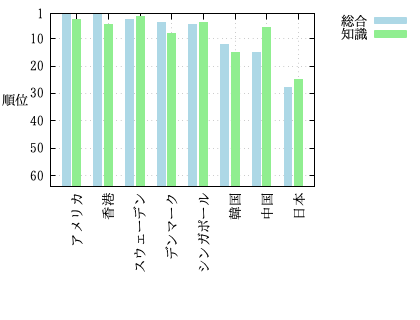
\includegraphics{fig31.png}
    \caption{デジタル競争力ランキング(64カ国中)}
    \label{fig:ranking}
\end{figure}
% \includegraphics{}
% を
% \begin{figure}[htbp]
% \end{figure}
% で囲み
% \caption{}
% で図のタイトルを入れる.
% \label{}
% を使って図番号が参照できるようにする
% また,
% \centering
% で図が中央に来るようにする

% ーーー
% 節見出し(2)

\section{ブロードバンドの整備状況}

OECDによるブロードバンド回線の普及に関する調査\cite{oecd}によると,表\ref{tbl:bb}に示すように,
日本におけるモバイルブロードバンドの加入者数は 190.5で,第1位になっている.2位はエストニアで,3位米国と続く.
% 本文(2)

% 表の挿入
\begin{table}[htbp]
    \centering
    \caption{モバイルブロードバンドの加入者数(100人あたり)}
    \label{tbl:bb}
    \begin{tabular}{|c|l|r|}
        \hline
        順位 & 国名 & 加入者数 \\\hline
        1位 & 日本 & 190.5 \\\hline
        2位 & エストニア & 179.9 \\\hline
        3位 & 米国 & 169.0 \\\hline
        4位 & フィンランド & 157.0 \\\hline
        5位 & デンマーク & 141.7 \\\hline
        6位 & ラトビア & 141.6 \\\hline
        7位 & イスラエル & 139.9 \\\hline
        8位 & オランダ & 133.7\\\hline
        9位 & ポーランド & 131.3\\\hline
        10位 & スウェーデン & 127.2\\\hline
    \end{tabular}
\end{table}
% \begin{tabular}
% \end{tabular}    
% による表の記述を 
% \begin{table}[htbp]
% \end{table}
% で囲み
% \caption{}
% で表のタイトルを入れる.
% \label{}
% を使って表番号が参照できるようにする
% また,
% \centering
% で表が中央に来るようにする

% ーーー
% 見出し(3)
% 考察
\section{考察}


%
% \begin{itemize}
% \end{itemize}
% を使って箇条書きで記述する

% ここに参考文献が入る
%
\bibliographystyle{junsrt}
\bibliography{exercise.bib}

\end{document}